%%%%%%%%%%%%%%%%%%%%%%%%%%%%%%%%%%%%%
%% Supporting Information
%% (Optional)
%%%%%%%%%%%%%%%%%%%%%%%%%%%%%%%%%%%%%
% OVERVIEW
%
% Please note that all supporting information will be peer reviewed with your manuscript.
% In general, the purpose of the supporting information is to enable
% authors to provide and archive auxiliary information such as data
% tables, method information, figures, video, or computer software,
% in digital formats so that other scientists can use it.

% The key criteria are that the data:
% 1. supplement the main scientific conclusions of the paper but are not essential to the conclusions (with the exception of
%    including data so the experiment can be reproducible);
% 2. are likely to be usable or used by other scientists working in the field;
% 3. are described with sufficient precision that other scientists can understand them, and
% 4. are not exe files.
%

% All Supporting text and figures should be included in this document.

% Data sets, large tables, movie files,
% and audio files should be uploaded separately, following AGU naming
% conventions. Include their captions in this document and list the
% file name with the caption. You will be prompted to upload these
% files on the Upload Files tab during the submission process, using
% file type “Supporting Information (SI)”

\documentclass[draft]{agujournal}

% Please type in the journal name: \journalname{<Journal Name>}
% ie,
\journalname{Journal of Geophysical Research}

%% Choose from this list of Journals:
%
% Journal of Geophysical Research
% JGR-Biogeosciences
% JGR-Earth Surface
% JGR-Planets
% JGR-Solid Earth
% JGR-Space Physics
% Global Biochemical Cycles
% Geophysical Research Letters
% Paleoceanography
% Radio Science
% Reviews of Geophysics
% Tectonics
% Space Weather
% Water Resource Research
% Geochemistry, Geophysics, Geosystems
% Journal of Advances in Modeling Earth Systems (JAMES)
% Earth's Future
% Earth and Space Science

\usepackage{gensymb} % To write degrees symbol as \degree
\usepackage{chemformula} % use \ch to write chemical formulas with automatic subscripting
\usepackage{array} % to fix table borders

\begin{document}

%% This command needs article title as argument to \supportinginfo{}:
\supportinginfo{Unexpected decreasing trend in formaldehyde detected from 20 year record at Wollongong, Southeast Australia}

\authors{Kaitlyn J. Lieschke\affil{1}\thanks{Current address, Department of Chemistry, University of California at Berkeley, Berkeley, CA, USA}, Jenny A. Fisher\affil{1,2}, Clare Paton-Walsh\affil{1}, Nicholas B. Jones\affil{1}, Jesse W. Greenslade\affil{1}, Sandy Burden\affil{3}, David W. T. Griffith\affil{1}}

\affiliation{1}{Centre for Atmospheric Chemistry, School of Chemistry, University of Wollongong, Wollongong, NSW, Australia}
\affiliation{2}{School of Earth and Environmental Sciences, University of Wollongong, Wollongong, NSW, Australia}
\affiliation{3}{National Institute for Applied Statistics Research Australia, School of Mathematics and Applied Statistics, University of Wollongong, Wollongong, NSW, Australia}

\correspondingauthor{Kaitlyn Lieschke}{kaitlyn\_lieschke@berkekey.edu}

%% ------------------------------------------------------------------------ %%
%
%  TEXT
%
%% ------------------------------------------------------------------------ %%

\section*{Contents}
%%%Remove or add items as needed%%%
\begin{enumerate}
\item Text S1 to S2
\item Figures S1 to S2
\item Table S1
\end{enumerate}

%\section*{Additional Supporting Information (Files uploaded separately)}

%\begin{enumerate}
%\item Captions for Datasets S1 to Sx
%\item Captions for large Tables S1 to Sx (if larger than 1 page, upload as separate excel file)
%\item Captions for Movies S1 to Sx
%\item Captions for Audio S1 to Sx
%\end{enumerate}

%Delete all unused file types below. 
%Copy/paste for multiples of each file type as needed.
\renewcommand\thefigure{S\arabic{figure}} %Set figures to be labelled as S1, S2 etc.
\renewcommand\thetable{S\arabic{table}} %Set table to be labelled as S1, S2 etc.

\section*{Text S1.}

\subsection*{Measurement Details}

HCHO measurements were collected from the Fourier Transform Infrared Spectrometer (FTIR) at the Wollongong site of the Network for the Detection of Atmospheric Composition Change (NDACC), located at the University of Wollongong (34.45 \degree S, 150.88 \degree E, 30 m above sea level). Measurements began in May 1996 with a Bomem DA8 FTIR spectrometer, which had a maximum optical path difference of 250 cm, corresponding to a maximum resolution of 0.004 cm$^{-1}$ \citep{Rinsland2001,Griffith1998}. In 2007 the system was upgraded to a Bruker IFS 125/HR, which has an optical path difference of 257 cm$^{-1}$ \citep{Sussmann2011}. The total column abundance of HCHO was determined by simultaneously fitting three microwindow ranges (2778.43 - 2778.56 cm$^{-1}$, 2780.65 - 2781.11 cm$^{-1}$, and 2912.00 - 2912.30 cm$^{-1}$). The method was based on the procedure outlined in \citet{Jones2009}. The analysis code used was SFIT2 v3.94 \citep{Rinsland1998}, which has a forward model to describe the physics of the atmosphere, the FTIR instrument to produce an infrared spectrum and a semi-empirical optimal estimation approach \citep{Rodgers2000} for the inverse model. The atmosphere is divided into 48 vertical layers, whose thickness is based on pressure. The temperature-pressure profile for the SFIT2 forward model was based on the daily mean of 6-hourly reanalysis data from the National Center for Environmental Prediction (NCEP). The a priori profile for HCHO was based on a scaled version of the profile reported in \citet{Singh2001}, where the scaling factor was determined from the mean of a pre-fit to all Wollongong data. The water profile was taken from the daily mean NCEP data, while profiles for all other interfering gases were from the Whole Atmosphere Community Climate Model \citep{Marsh2013}. We use individual column retrievals made several times a day under clear sky conditions, subject to quality control, from May 1996 to December 2015. Trends for each month over this time period are calculated using the average of the retrievals within each month. As the FTIR is shared with the Total Column Carbon Observing Network (TCCON), NDACC measurements are made on approximately half of the available clear sky days.

Observations of temperature and wind around Wollongong were sourced from the Australian Bureau of Meteorology sites as listed in Table \ref{tab:sites}.

\begin{table}
\begin{center}
\begin{tabular}{ | l | l | l | }
  \hline
  \textbf{Site} & \textbf{Latitude} & \textbf{Longitude} \\  \hline
  Badgery's Creek & -33.8969 & 150.7281 \\  \hline
  Bankstown & -33.9181 & 150.9864 \\  \hline
  Bowral & -34.4869 & 150.4019 \\  \hline
  Nowra & -34.9449 & 150.5450 \\
   & -34.9469 & 150.5353 \\  \hline
  Penrith Lakes & -33.7195 & 150.6783 \\  \hline
  Prospect Reservoir & -33.8193 & 150.9127 \\  \hline
\end{tabular}
\caption{Latitude and longitude of Australian Bureau of Meteorology sites used in temperature analysis.}
\label{tab:sites}
\end{center}
\end{table}

The OMI instrument is onboard the NASA Aqua satellite, which has a local overpass time of 1330, resulting in approximately 1-2 swaths over Wollongong per day. OMI uses two-dimensional charge-coupled devices (CCD) to measure back-scattered solar UV radiation from 270-500 nm. HCHO is measured in the UV-2 channel ranging from 307-383 nm with a spectral resolution of 0.63 nm \citep{Gonzalez2015}. Estimates of HCHO total column were extracted from OMIHCHO daily swath data using the reference sector corrections described in \citet{Gonzalez2015}. Pixels with non-zero main data quality flag, non-zero cross track anomaly flag, cloud fraction over 40\% and pixels centred over ocean were removed. In addition to this, measurements were  filtered according to \citet{Zhu2016} to exclude values outside of the range -5$\cdot$10$^{15}$ to 1$\cdot$10$^{17}$, as well as any with a solar zenith angle greater than 60\degree. The remaining pixels were screened by location and averaged over three regions of Australia to give total column averages for a given region (see Figure 1). The regions were: 33.5-35.5 \degree S x 150.0-151.5 \degree E (South Coast), 32-36 \degree S x 147.5-152.5 \degree E (GEOS-Chem) and 30-38 \degree S x 145-153 \degree E (South-East Australia).

\section*{Text S2.}

\subsection*{Model description}

We simulate HCHO over southeast Australia using the GEOS-Chem v9-02 chemical transport model driven by assimilated meteorology from the Modern-Era Retrospective Analysis for Research and Applications (MERRA) NASA Global Modelling and Assimilation Office \citep{Bey2001,Rienecker2011}. The native MERRA horizontal resolution of 0.5 \degree x 0.667 \degree was downgraded to 4$\degree$ x 5$\degree$ to enable a 15 year simulation, with a vertical resolution of 47 vertical levels. Transport and convection were calculated on 30 min time steps, and emissions and chemistry were calculated on 60 min time steps.

Biogenic NMVOC emissions are from the Model of Emissions of Gases and Aerosols from Nature version 2.1 (MEGAN2.1) \citep{Guenther2012}. Anthropogenic emissions are from the Emissions Database for Global Atmospheric Research version 3.2 (EDGAR3.2) for \ch{CO2}, \ch{NOx} and \ch{SO2} \citep{Olivier2005} and the Reanalysis of the Tropospheric Chemical Composition version 2 (RETRO2) for NMVOCs \citep{Hu2015}. Biomass burning emissions are from the Global Fire Emissions Database version 3 (GFED3) with monthly temporal resolution \citep{VanDerWerf2010}.

The model was run from 1997 to 2011, with the time span limited by the availability of biomass burning input from GFED3. The output was convolved with FTIR averaging kernels and a priori before comparison \citep{Rodgers2003}.

FTIR retrievals were converted to daily averages for comparison with model output and then to monthly averages for monthly trends.

\subsection*{Model Comparison}

Figure \ref{fig:gc_ts} shows the (A) timeseries and (B) seasonal cycle of the daily mean HCHO total column abundance at Wollongong according to both FTIR observations (blue) and GEOS-Chem simulations (red). The model reproduces much of the variability in the measurements with a correlation coefficient of 0.66 and a mean bias of -7.3$\cdot$10$^{15}$ molecs cm$^{-1}$. This bias is consistent with a previous model evaluation at Wollongong by \citet{Zeng2015} who found that four different models (including GEOS-Chem) underestimate HCHO abundance at Wollongong. They suggested this bias was due to missing direct and indirect sources from nearby Sydney, missing chemical processes in the models or a combination of these factors. 

\begin{figure}[h!]
  \begin{center}
    \includegraphics[width=0.7\textwidth]{HCHO_OE_GC_timeseries_Wollongong_edited}
      \caption{HCHO total columns from FTIR observations (blue) and GEOS-Chem simulations (red) at Wollongong, southeast Australia from 1997-2011 showing (A) the long term time series and (B) the average seasonal cycle, along with associated 95\% confidence interval shown by the shaded regions.}
  \label{fig:gc_ts}
  \end{center}
\end{figure}

When limited to the period of time simulated by GEOS-Chem (1997-2011) the FTIR showed a decrease of -1.83 [-2.76, -0.57]\% yr$^{-1}$ in HCHO, while the model simulated no significant trend. The model bias changes over time, but this change is consistent with the trend observed in the FTIR so should not impact further analysis. Figure \ref{fig:gc_trends} shows the calculated trends in monthly HCHO abundance during this period from measurements (blue) and convolved model values (red). Over this shorter time window, fewer months show significant trends in the FTIR data with decreases observed in March, April, June, July, August, September, October and December. The difference from Figure 3 is not due to the different averaging times used in the two calculations (individual retrievals vs daily means) as we find the same observed trends when individual retrieval information is used rather than daily means.

\begin{figure}[h!]
  \begin{center}
    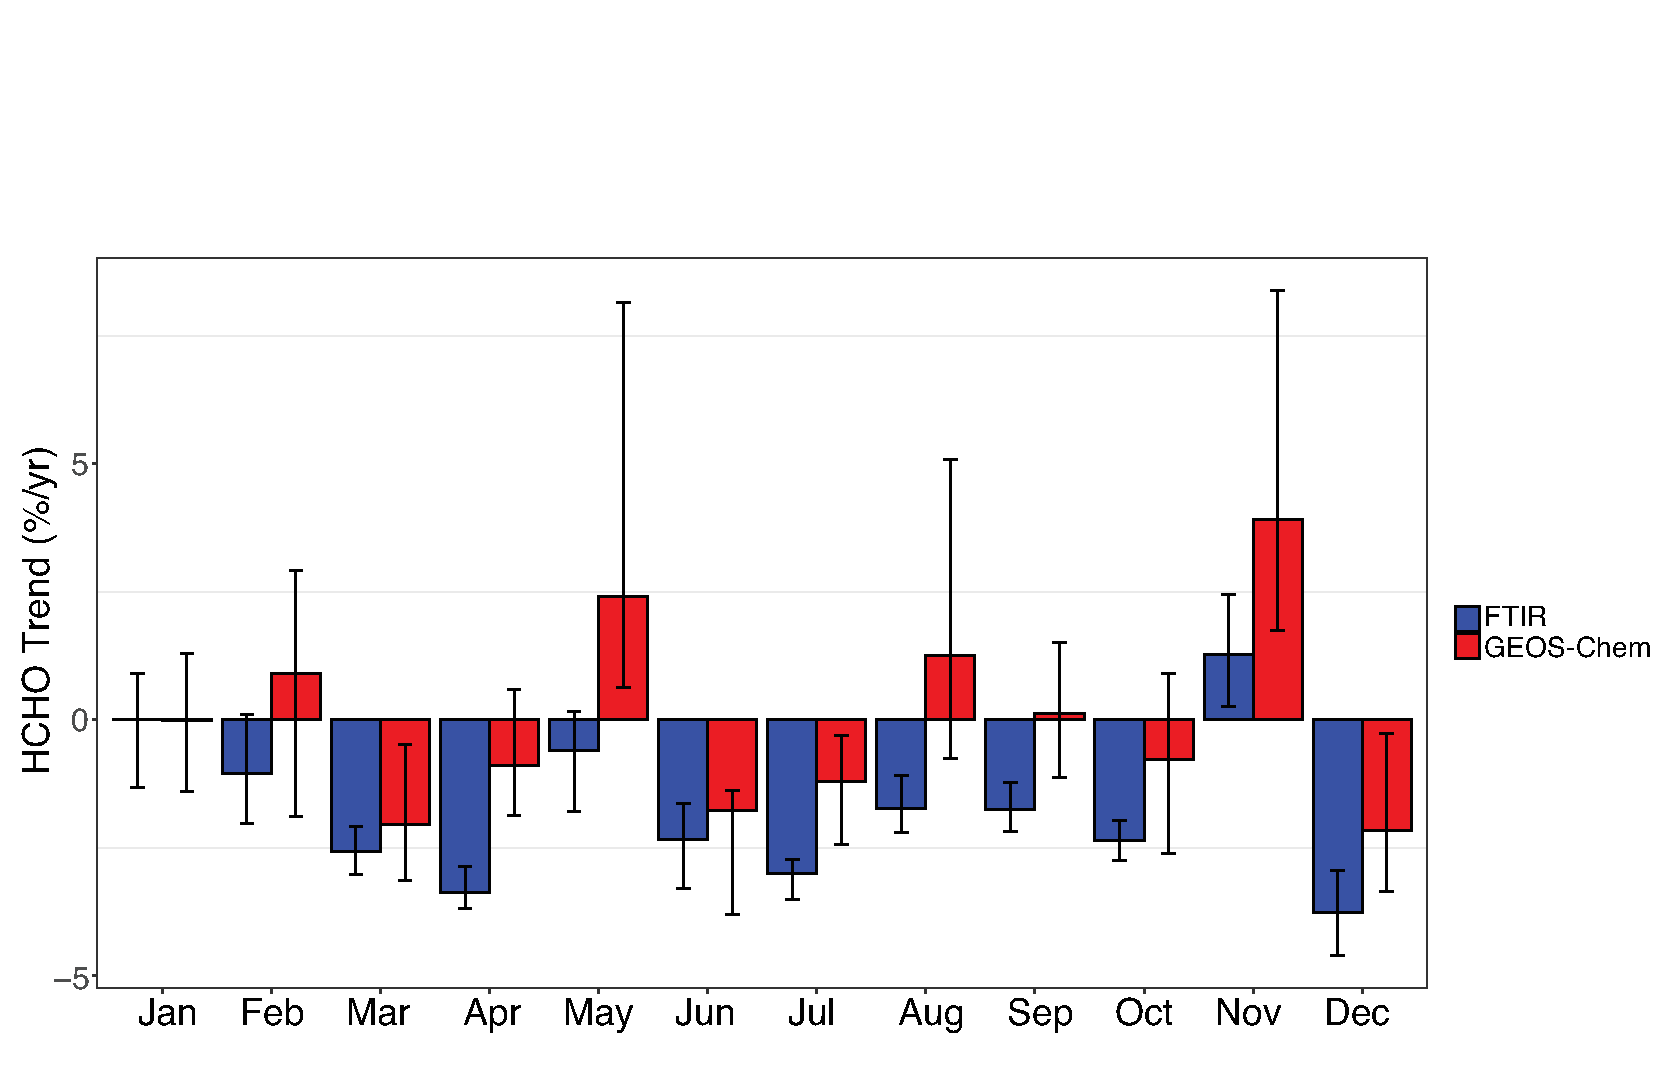
\includegraphics[width=0.75\textwidth]{HCHO_OE_GC_Monthly_Trends_Wollongong}
      \caption{Monthly trends in HCHO total columns from FTIR observations (blue) and GEOS-Chem simulations (red) at Wollongong, South-East Australia from 1997-2011, along with associated 95\% confidence interval.}
  \label{fig:gc_trends}
  \end{center}
\end{figure}

GEOS-Chem well represents the decreases in March, June, July and December but is unable to simulate the significant trends observed in April, August, September and October. The observations also suggest an increasing trend in November which is simulated by the model, however the model also simulates a significant increase in May which was not observed. These discrepancies, as well as the negative bias in the simulations, could be caused by the large size of the model grid box containing Wollongong. This could cause local effects to be smeared out or the grid box abundance to be dominated by other factors, further supporting the suggestion that local effects at Wollongong are causing the observed decrease in HCHO. Another factor affecting the simulations could be that the isoprene emission rates built into MEGAN2.1 are not appropriate for 
the environmental conditions at Wollongong, as noted by \citet{Emmerson2016}.

%\section*{Data Set S1.} %Type or paste caption here.
%
%Upload your dataset(s) to AGU's journal submission site and select
%"Supporting Information (SI)" as the file type. Following naming
%convention: ds01.
%
%Repeat for any additional Supporting data sets
%
%\section*{Movie S1.} 
%
%Type or paste caption here.
%
%Upload your movie(s) to AGU's journal submission site and select,
%"Supporting Information (SI)" as the file type. Following naming convention: ms01.
%
%Repeat any additional Supporting movies
%
%\section*{Audio S1.} 
%
%Type or paste caption here.
%
%Upload your audio file(s) to AGU's journal submission site and select
%Supporting Information ``(SI)" as the file type. Following naming
%convention: auds01.
%
%Repeat for any additional Supporting audio files

%\bibliography{formaldehydesi}

\begin{thebibliography}{19}
\providecommand{\natexlab}[1]{#1}
\expandafter\ifx\csname urlstyle\endcsname\relax
  \providecommand{\doi}[1]{doi:\discretionary{}{}{}#1}\else
  \providecommand{\doi}{doi:\discretionary{}{}{}\begingroup
  \urlstyle{rm}\Url}\fi

\bibitem[{\textit{Bey et~al.}(2001)\textit{Bey, Jacob, Yantosca, Logan, Field,
  Fiore, Li, Liu, Mickley, and Schultz}}]{Bey2001}
Bey, I., D.~J. Jacob, R.~M. Yantosca, J.~a. Logan, B.~D. Field, A.~M. Fiore,
  Q.~Li, H.~Liu, L.~J. Mickley, and M.~G. Schultz (2001), {Global modeling of
  tropospheric chemistry with assimilated meteorology: Model description and
  evaluation}, \textit{Journal of Geophysical Research}, \textit{106},
  23,073--23,095, \doi{10.1029/2001JD000807}.

\bibitem[{\textit{Emmerson et~al.}(2016)\textit{Emmerson, Galbally, Guenther,
  Paton-Walsh, Guerette, Cope, Keywood, Lawson, Molloy, Dunne, Thatcher, Karl,
  and Maleknia}}]{Emmerson2016}
Emmerson, K.~M., I.~E. Galbally, A.~B. Guenther, C.~Paton-Walsh, E.-A.
  Guerette, M.~E. Cope, M.~D. Keywood, S.~J. Lawson, S.~B. Molloy, E.~Dunne,
  M.~Thatcher, T.~Karl, and S.~D. Maleknia (2016), {Current estimates of
  biogenic emissions from eucalypts uncertain for southeast Australia},
  \textit{Atmospheric Chemistry and Physics}, \textit{16}, 6997--7011,
  \doi{10.5194/acp-16-6997-2016}.

\bibitem[{\textit{{Gonz{\'{a}}lez Abad} et~al.}(2015)\textit{{Gonz{\'{a}}lez
  Abad}, Liu, Chance, Wang, Kurosu, and Suleiman}}]{Gonzalez2015}
{Gonz{\'{a}}lez Abad}, G., X.~Liu, K.~Chance, H.~Wang, T.~P. Kurosu, and
  R.~Suleiman (2015), {Updated Smithsonian Astrophysical Observatory Ozone
  Monitoring Instrument (SAO OMI) formaldehyde retrieval}, \textit{Atmospheric
  Measurement Techniques}, \textit{8}, 19--32, \doi{10.5194/amt-8-19-2015}.

\bibitem[{\textit{Griffith et~al.}(1998)\textit{Griffith, Jones, and
  Matthews}}]{Griffith1998}
Griffith, D. W.~T., N.~B. Jones, and W.~A. Matthews (1998), {Interhemispheric
  ratio and annual cycle of carbonyl sulfide (OCS) total column from
  ground-based solar FTIR spectra}, \textit{Journal of Geophysical Research},
  \textit{103}(D7), 8447, \doi{10.1029/97JD03462}.

\bibitem[{\textit{Guenther et~al.}(2012)\textit{Guenther, Jiang, Heald,
  Sakulyanontvittaya, Duhl, Emmons, and Wang}}]{Guenther2012}
Guenther, A.~B., X.~Jiang, C.~L. Heald, T.~Sakulyanontvittaya, T.~Duhl, L.~K.
  Emmons, and X.~Wang (2012), {The Model of Emissions of Gases and Aerosols
  from Nature version 2.1 (MEGAN2.1): an extended and updated framework for
  modeling biogenic emissions}, \textit{Geoscientific Model Development},
  \textit{5}, 1471--1492, \doi{10.5194/gmd-5-1471-2012}.

\bibitem[{\textit{Hu et~al.}(2015)\textit{Hu, Millet, Baasandorj, Griffis,
  Travis, Tessum, Marshall, Reinhart, Mikoviny, M{\"{u}}ller, Wisthaler, Graus,
  Warneke, and de~Gouw}}]{Hu2015}
Hu, L., D.~B. Millet, M.~Baasandorj, T.~J. Griffis, K.~R. Travis, C.~W. Tessum,
  J.~D. Marshall, W.~F. Reinhart, T.~Mikoviny, M.~M{\"{u}}ller, A.~Wisthaler,
  M.~Graus, C.~Warneke, and J.~de~Gouw (2015), {Emissions of C6-C8 aromatic
  compounds in the United States: Constraints from tall tower and aircraft
  measurements}, \textit{Journal of Geophysical Research: Atmospheres},
  \textit{120}, 826--842, \doi{10.1002/2014JD022627.Received}.

\bibitem[{\textit{Jones et~al.}(2009)\textit{Jones, Riedel, Allan, Wood,
  Palmer, Chance, and Notholt}}]{Jones2009}
Jones, N.~B., K.~Riedel, W.~Allan, S.~Wood, P.~I. Palmer, K.~Chance, and
  J.~Notholt (2009), {Long-term tropospheric formaldehyde concentrations
  deduced from ground-based fourier transform solar infrared measurements},
  \textit{Atmospheric Chemistry and Physics}, \textit{9}, 7131--7142,
  \doi{10.5194/acpd-7-14543-2007}.

\bibitem[{\textit{Marsh et~al.}(2013)\textit{Marsh, Mills, Kinnison, Lamarque,
  Calvo, and Polvani}}]{Marsh2013}
Marsh, D.~R., M.~J. Mills, D.~E. Kinnison, J.-F. Lamarque, N.~Calvo, and L.~M.
  Polvani (2013), {Climate change from 1850 to 2005 simulated in CESM1(WACCM)},
  \textit{Journal of Climate}, \textit{26}, 7372--7391,
  \doi{10.1175/JCLI-D-12-00558.1}.

\bibitem[{\textit{Olivier et~al.}(2005)\textit{Olivier, {Van Aardenne},
  Dentener, Pagliari, Ganzeveld, and Peters}}]{Olivier2005}
Olivier, J. G.~J., J.~a. {Van Aardenne}, F.~J. Dentener, V.~Pagliari, L.~N.
  Ganzeveld, and J.~a. H.~W. Peters (2005), {Recent trends in global greenhouse
  gas emissions:regional trends 1970-2000 and spatial distributionof key
  sources in 2000}, \textit{Environmental Sciences}, \textit{2}, 81--99,
  \doi{10.1080/15693430500400345}.

\bibitem[{\textit{Rienecker et~al.}(2011)\textit{Rienecker, Suarez, Gelaro,
  Todling, Bacmeister, Liu, Bosilovich, Schubert, Takacs, Kim, Bloom, Chen,
  Collins, Conaty, {Da Silva}, Gu, Joiner, Koster, Lucchesi, Molod, Owens,
  Pawson, Pegion, Redder, Reichle, Robertson, Ruddick, Sienkiewicz, and
  Woollen}}]{Rienecker2011}
Rienecker, M.~M., M.~J. Suarez, R.~Gelaro, R.~Todling, J.~Bacmeister, E.~Liu,
  M.~G. Bosilovich, S.~D. Schubert, L.~Takacs, G.~K. Kim, S.~Bloom, J.~Chen,
  D.~Collins, A.~Conaty, A.~{Da Silva}, W.~Gu, J.~Joiner, R.~D. Koster,
  R.~Lucchesi, A.~Molod, T.~Owens, S.~Pawson, P.~Pegion, C.~R. Redder,
  R.~Reichle, F.~R. Robertson, A.~G. Ruddick, M.~Sienkiewicz, and J.~Woollen
  (2011), {MERRA: NASA's modern-era retrospective analysis for research and
  applications}, \textit{Journal of Climate}, \textit{24}, 3624--3648,
  \doi{10.1175/JCLI-D-11-00015.1}.

\bibitem[{\textit{Rinsland et~al.}(1998)\textit{Rinsland, Jones, Connor, Logan,
  Pougatchev, Goldman, Murcray, Stephen, Pine, Zander, Mahieu, and
  Demoulin}}]{Rinsland1998}
Rinsland, C.~P., N.~B. Jones, B.~J. Connor, J.~a. Logan, N.~S. Pougatchev,
  A.~Goldman, F.~J. Murcray, T.~M. Stephen, A.~S. Pine, R.~Zander, E.~Mahieu,
  and P.~Demoulin (1998), {Northern and southern hemisphere ground-based
  infrared spectroscopic measurements of tropospheric carbon monoxide and
  ethane}, \textit{Journal of Geophysical Research}, \textit{103},
  28,197--28,217.

\bibitem[{\textit{Rinsland et~al.}(2001)\textit{Rinsland, Meier, Griffith, and
  Chiou}}]{Rinsland2001}
Rinsland, C.~P., A.~Meier, D.~W.~T. Griffith, and L.~S. Chiou (2001),
  {Ground-based measurements of tropospheric CO, C2H6, and HCN from Australia
  at 34 degrees S latitude during 1997-1998}, \textit{Journal of Geophysical
  Research}, \textit{106}, 20,913--20,924, \doi{10.1029/2000JD000318}.

\bibitem[{\textit{Rodgers}(2000)}]{Rodgers2000}
Rodgers, C.~D. (2000), {Error Analysis and Characterisation}, in
  \textit{Inverse Methods for Atmospheric Sounding: Theory and Practice},
  chap.~3, pp. 43--63, World Scientific Publishing Co. Pte. Ltd., Singapore.

\bibitem[{\textit{Rodgers and Connor}(2003)}]{Rodgers2003}
Rodgers, C.~D., and B.~J. Connor (2003), {Intercomparison of remote sounding
  instruments}, \textit{Journal of Geophysical Research}, \textit{108}(D3), ACH
  13--1 -- ACH 13--14, \doi{10.1029/2002JD002299}.

\bibitem[{\textit{Singh et~al.}(2001)\textit{Singh, Chen, Staudt, Jacob, Blake,
  Heikes, and Snow}}]{Singh2001}
Singh, H., Y.~Chen, A.~Staudt, D.~Jacob, D.~Blake, B.~Heikes, and J.~Snow
  (2001), {Evidence from the Pacific troposphere for large global sources of
  oxygenated organic compounds.}, \textit{Nature}, \textit{410}, 1078--1081,
  \doi{10.1038/35074067}.

\bibitem[{\textit{Sussmann et~al.}(2011)\textit{Sussmann, Forster, Rettinger,
  and Jones}}]{Sussmann2011}
Sussmann, R., F.~Forster, M.~Rettinger, and N.~Jones (2011), {Strategy for
  high-accuracy-and-precision retrieval of atmospheric methane from the
  mid-infrared FTIR network}, \textit{Atmospheric Measurement Techniques},
  \textit{4}, 1943--1964, \doi{10.5194/amt-4-1943-2011}.

\bibitem[{\textit{{Van Der Werf} et~al.}(2010)\textit{{Van Der Werf},
  Randerson, Giglio, Collatz, Mu, Kasibhatla, Morton, Defries, Jin, and {Van
  Leeuwen}}}]{VanDerWerf2010}
{Van Der Werf}, G.~R., J.~T. Randerson, L.~Giglio, G.~J. Collatz, M.~Mu, P.~S.
  Kasibhatla, D.~C. Morton, R.~S. Defries, Y.~Jin, and T.~T. {Van Leeuwen}
  (2010), {Global fire emissions and the contribution of deforestation,
  savanna, forest, agricultural, and peat fires (1997-2009)},
  \textit{Atmospheric Chemistry and Physics}, \textit{10}, 11,707--11,735,
  \doi{10.5194/acp-10-11707-2010}.

\bibitem[{\textit{Zeng et~al.}(2015)\textit{Zeng, Williams, Fisher, Emmons,
  Jones, Morgenstern, Robinson, Smale, Paton-Walsh, and Griffith}}]{Zeng2015}
Zeng, G., J.~E. Williams, J.~A. Fisher, L.~K. Emmons, N.~B. Jones,
  O.~Morgenstern, J.~Robinson, D.~Smale, C.~Paton-Walsh, and D.~W.~T. Griffith
  (2015), {Multi-model simulation of CO and HCHO in the Southern Hemisphere:
  comparison with observations and impact of biogenic emissions},
  \textit{Atmospheric Chemistry and Physics}, \textit{15}(13), 7217--7245,
  \doi{10.5194/acp-15-7217-2015}.

\bibitem[{\textit{Zhu et~al.}(2016)\textit{Zhu, Jacob, Kim, Fisher, Yu, Travis,
  Mickley, Yantosca, Sulprizio, {De Smedt}, Abad, Chance, Li, Ferrare, Fried,
  Hair, Hanisco, Richter, Scarino, Walega, Weibring, and Wolfe}}]{Zhu2016}
Zhu, L., D.~J. Jacob, P.~S. Kim, J.~A. Fisher, K.~Yu, K.~R. Travis, L.~J.
  Mickley, R.~M. Yantosca, M.~P. Sulprizio, I.~{De Smedt}, G.~G. Abad,
  K.~Chance, C.~Li, R.~Ferrare, A.~Fried, J.~W. Hair, T.~F. Hanisco,
  D.~Richter, A.~J. Scarino, J.~Walega, P.~Weibring, and G.~M. Wolfe (2016),
  {Observing atmospheric formaldehyde (HCHO) from space: Validation and
  intercomparison of six retrievals from four satellites (OMI, GOME2A, GOME2B,
  OMPS) with SEAC4RS aircraft observations over the southeast US},
  \textit{Atmospheric Chemistry and Physics}, \textit{16}(21), 13,477--13,490,
  \doi{10.5194/acp-16-13477-2016}.

\end{thebibliography}

\end{document}